\documentclass[12pt]{article}
\usepackage[right=1.25in,left=1.25in,top=1.1in,bottom=1.1in]{geometry}
\usepackage{hyperref}
\hypersetup{colorlinks, citecolor=blue, filecolor=blue, linkcolor=blue, urlcolor=blue}
\usepackage{graphicx}
\usepackage{url}
\usepackage[round]{natbib}
\usepackage{amsmath,amsthm} 
\usepackage{engord}
\usepackage{float}
\usepackage{subfig}
\usepackage{pdflscape}
\usepackage{booktabs}
\usepackage{pgfplots}
\pgfplotsset{compat=1.18}
\pgfplotsset{every axis label/.append style={font=\tiny}}
\usepackage[labelsep=period]{caption} %% This switches "Table 1: Title" to "Table 1. Title"
\usepackage{tikz}
\usepackage{graphicx}
\usepackage{amssymb} %% Necessary, just for the \checkmark command  in tables.
\usepackage{multirow} %% Necessary if we are doing tables in LaTeX
% \usepackage{subfigure}
% \usepackage{subcaption}
\usepackage{xr}

\usepackage{setspace}
\onehalfspacing

\usepackage{sectsty}
\sectionfont{\large}
\subsectionfont{\normalsize}
\subsubsectionfont{\normalsize}

\newcommand{\specialcell}[2][c]{\begin{tabular}[#1]{@{}l@{}}#2\end{tabular}}

%%%%%%%%%%%%%%%%%%%%%%%%%%%%%%%%%%%%%%%%%%%%%%%%%%%%%%%%%%%%%

\title{ \vspace*{-2.5cm} \hspace*{-0.5cm}Pricing Tail Risk: \\ A Structured Mixture Density Network Approach\footnote{
nan
}}

\author{Jianbin Chen\thanks{University of California, Riverside.
\href{mailto:jchen939@ucr.edu}{jchen939@ucr.edu}} }

\date{ \vspace*{0.5cm} June, 2026\\
\textbf{Job Market Paper \\ Preliminary and Incomplete. \\ Please do not cite or circulate.}
} 

%%%%%%%%%%%%%%%%%%%%%%%%%%%%%%%%%%%%%%%%%%%%%%%%%%%%%%%%%%%%%

\begin{document}

\bgroup
\let\footnoterule\relax

\begin{singlespace}
\maketitle


\begin{abstract}
    \noindent Pending.
\end{abstract}
\end{singlespace}
\thispagestyle{empty}

\clearpage
\egroup
\setcounter{page}{1}

%% Temporary tool to track how this paper is structured. Feel free to comment in or out. 
% \tableofcontents
% \bigskip

%%%%%%%%%%%%%%%%%%%%%%%%%%%%%%%%%%%%%%%%%%%%%%%%%%%%%%%%%%%%%
%%%%\section{Introduction\label{sec:introduction}}

\noindent Introduction

We also cite papers in this document \citep{Chetty2013}. For instance: \citet{Hansen1992}. So on and so forth\ldots

The remainder of the paper proceeds as follows. Section \ref{sec:background} provides background. We then present our
empirical results in Section \ref{sec:results}. Finally, Section \ref{sec:conclusion} concludes. 

\section{Background \label{sec:background}}

In the past, people only estimate the $E[R]$. It it not enough. Now we need to estimate the density to help us find the left tail risk. 

\begin{figure}[htbp]
    \begin{center}
    \caption{mixture density example}
    \label{fig:fig_mixture_density_example}
    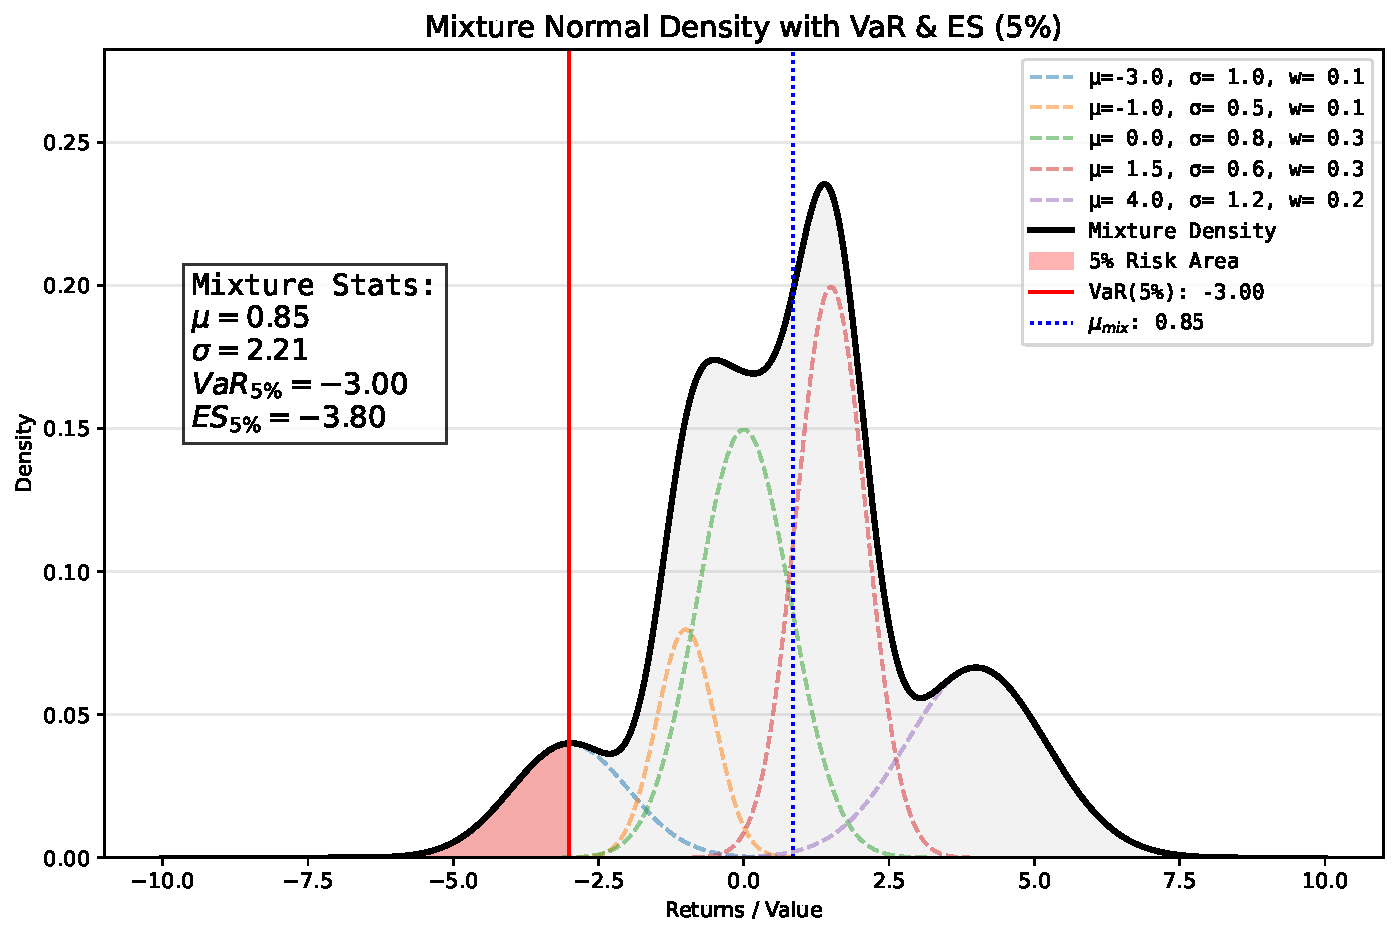
\includegraphics[width=1\textwidth]{fig/slice_3_final_var.pdf}
    \end{center}
    % \vspace{0.2cm}
 %    \begin{minipage}{0.95\textwidth} 
	% {\footnotesize This figure plots \ldots
	% \par
	% }
	% \end{minipage}
\end{figure}


Figure \ref{fig:fig_mixture_density_example} .

Based on the density, we can calculate the value at risk and expected shortfall. 



\section{Theoretical Derivation}

\subsection{Step 1: The Representative Investor's Utility Maximization Problem}

Consider a representative investor with wealth $W_t$. In traditional mean-variance or standard Constant Relative Risk Aversion (CRRA) utility frameworks, the investor's risk aversion is smooth across all states. To introduce tail risk pricing, we assume the investor's utility function incorporates an additional \textbf{tail penalty} for extreme downside risk.

Let the next-period wealth be $W_{t+1} = W_t R_{m,t+1}$, where $R_{m,t+1}$ is the gross return of the market portfolio. The investor's utility function is defined as:

$$U(W_{t+1}) = \frac{W_{t+1}^{1-\gamma}}{1-\gamma} - \kappa \max(0, W_t \tau - W_{t+1})$$

where:
\begin{itemize}
    \item $\gamma$ is the coefficient of relative risk aversion (RRA).
    \item $\tau$ is the return threshold that triggers a ``crash'' state (e.g., a market drop of more than 5\% implies $\tau = 0.95$).
    \item $\kappa > 0$ is the tail aversion parameter, capturing the investor's additional panic or distress from liquidity constraints when the return falls below the threshold.
\end{itemize}

The investor's optimization problem is to choose the investment weight for asset $i$ to maximize expected utility. According to the first-order condition (Euler Equation), for the gross return $R_{i,t+1}$ of any risky asset $i$, the following must hold:

$$E_t [\beta U'(W_{t+1}) R_{i,t+1}] = U'(W_t)$$

\subsection{Step 2: Deriving the Tail-Sensitive SDF}

We rewrite the above Euler equation into the standard pricing form using the Stochastic Discount Factor (SDF, $M_{t+1}$):

$$E_t [M_{t+1} R_{i,t+1}] = 1$$

where $M_{t+1} = \beta \frac{U'(W_{t+1})}{U'(W_t)}$.

Differentiating the utility function defined in Step 1, we obtain the marginal utility for the next period:

$$U'(W_{t+1}) = W_{t+1}^{-\gamma} + \kappa \mathbf{1}_{\{R_{m,t+1} < \tau\}}$$

Here, $\mathbf{1}_{\{ \cdot \}}$ is the indicator function, which takes the value of 1 when the market return falls below the threshold $\tau$, and 0 otherwise.

Substituting $W_{t+1} = W_t R_{m,t+1}$ and applying a Taylor expansion (assuming $\gamma$ is reasonably small or using a log-linear approximation) to extract the linear components, we can approximate the SDF as a two-factor affine structure:

$$M_{t+1} \approx a - b R_{m,t+1} + \lambda \mathbf{1}_{\{R_{m,t+1} < \tau\}}$$

where:
\begin{itemize}
    \item $a, b > 0$ are parameters corresponding to the traditional CAPM dimension (representing smooth market risk).
    \item $\lambda \propto \kappa$ is the \textbf{Tail State Price Density}. It indicates that when a market crash occurs ($R_{m,t+1} < \tau$), the SDF experiences a non-linear upward jump. Marginal utility is exceptionally high in this state, making one unit of payoff extremely valuable.
\end{itemize}

\subsection{Step 3: Decomposition of the Cross-Sectional Risk Premium}

According to the fundamental theorem of asset pricing, the expected excess return of asset $i$ can be expressed as the covariance between its excess return $R_{i,t+1}^e$ and the SDF:

$$E_t[R_{i,t+1}^e] = -R_f \text{Cov}_t(M_{t+1}, R_{i,t+1}^e)$$

Substituting our tail-sensitive SDF into the covariance formula yields:

$$E_t[R_{i,t+1}^e] = R_f \cdot b \cdot \text{Cov}_t(R_{m,t+1}, R_{i,t+1}^e) - R_f \cdot \lambda \cdot \text{Cov}_t(\mathbf{1}_{\{R_{m,t+1} < \tau\}}, R_{i,t+1}^e)$$

This equation elegantly decomposes the expected excess return into two components:
\begin{enumerate}
    \item \textbf{The first term (Traditional Market Risk Premium):} The compensation an asset receives for covarying with overall market fluctuations (traditional Beta).
    \item \textbf{The second term (Tail Risk Premium):} This is the core focus of our study. Since $\lambda > 0$, to maintain the equality, if an asset exhibits exceptionally poor returns during a market crash ($\mathbf{1} = 1$)—meaning the covariance is large and negative in absolute terms—this term will generate a substantial \textbf{positive risk premium}.
\end{enumerate}

\subsection{Step 4: The Theoretical Bridge from Covariance to Dynamic Expected Shortfall (ES)}

We now map the covariance term $\text{Cov}_t(\mathbf{1}, R_i)$ from our theoretical model to the \textbf{dynamic Expected Shortfall ($ES_{i,t}$)} predicted by the MDN.

By definition, the conditional $ES$ of an individual stock is the lower tail expectation:

$$ES_{i,t}(\alpha) = - E_t [ R_{i,t+1} | R_{i,t+1} \le VaR_{i,t}(\alpha) ]$$

An established empirical fact in financial markets is that extreme downturns in individual stocks are often accompanied by extreme market downturns (i.e., \textbf{Lower Tail Dependence}). Therefore, a larger $ES_{i,t}$ for a stock (meaning it suffers more severe losses during its own tail events) implies a more negative conditional expected return during a market crash state ($R_{m,t+1} < \tau$):

$$E_t [ R_{i,t+1}^e | R_{m,t+1} < \tau ] \approx - \theta \cdot ES_{i,t}(\alpha)$$

where $\theta > 0$ is a mapping coefficient.

Substituting this conditional expectation back into the covariance term from Step 3 (utilizing the conditional expectation decomposition property of covariance), we ultimately derive a testable linear relationship for cross-sectional expected returns:

$$E_t[R_{i,t+1}^e] = \beta_{i,t}^{mkt} \lambda_{mkt} + \gamma_{tail} \cdot ES_{i,t}(\alpha)$$

\textbf{Conclusion of the Theoretical Derivation:} 
Because investors possess tail aversion to extreme states ($\kappa > 0 \implies \lambda > 0 \implies \gamma_{tail} > 0$), controlling for market Beta, \textbf{stocks with larger conditional $ES_{i,t}$ predicted by the MDN must offer higher expected excess returns in equilibrium.} This not only answers ``why ES should be priced,'' but also directly embeds the machine learning output variable, $ES_{i,t}$, into the macro-financial SDF.

\section{Data and Feature Engineering}
\label{sec:data_feature_engineering}

To estimate the conditional return density and extract accurate expected shortfall measures, we construct a comprehensive dataset combining firm-level micro characteristics and market-level macro predictors. Our sample spans from January 1990 to December 2023.

\subsection{Data Sources and Sample Selection}
\label{subsec:data_sources}

Our firm-level data is sourced from the Center for Research in Security Prices (CRSP) and the Compustat database via Wharton Research Data Services (WRDS). The CRSP database provides monthly stock prices, returns, and shares outstanding, while Compustat provides the accounting data necessary to construct fundamental ratios. Our initial universe includes all common stocks (share codes 10 and 11) traded on the NYSE, AMEX, and NASDAQ.

To ensure that our empirical results are driven by economically meaningful risk premiums rather than market friction, we impose a strict liquidity and tradability filter. Specifically, at the end of each portfolio formation month $t$, we exclude ``penny stocks'' with a closing price below \$5. This ex-ante exclusion is crucial for machine learning models, as extreme, noise-driven percentage returns of micro-cap stocks can heavily distort the optimization of the loss function (gradient hijacking) and introduce severe microstructure noise, such as the bid-ask bounce.

\subsection{Microeconomic Firm Characteristics}
\label{subsec:micro_features}

We employ a comprehensive set of firm-specific characteristics as inputs for the ``Expert Network'' of our Structured MDN. These variables encompass a wide spectrum of established asset pricing anomalies, including valuation ratios (e.g., Book-to-Market, Price-to-Earnings, Dividend Yield), profitability (e.g., ROE, Gross Profitability), momentum (e.g., 12-month trailing return), and trading frictions (e.g., Turnover, Size). 

Given the high dimensionality and the presence of extreme outliers in raw accounting data, directly feeding these values into a neural network often leads to instability and poor generalization. To address this, we apply a \textbf{Cross-Sectional Rank Normalization} procedure. For each characteristic $c$ at month $t$, we rank all eligible stocks and map the ranks into a continuous interval of $[-1, 1]$:
\begin{equation}
    \tilde{X}_{i,c,t} = \left( \frac{\text{Rank}(X_{i,c,t}) - 1}{N_t - 1} \right) \times 2 - 1
\end{equation}
where $N_t$ is the number of valid stocks in month $t$. Missing values for any characteristic are robustly imputed using the cross-sectional mean (which equals 0 after normalization). This non-parametric transformation preserves the ordinal cross-sectional ranking of the predictors while completely immunizing the network against extreme fundamental outliers.

\subsection{Macroeconomic Predictors}
\label{subsec:macro_features}

To capture shifts in the aggregate economic state and time-varying risk premiums, we utilize a set of macroeconomic predictors. The primary dataset is based on the classical variables compiled by , including the Term Spread (TMS), Default Yield Spread (DFY), Dividend Yield (D/Y), and Treasury Bill rates. Furthermore, to explicitly feed the network with systemic risk states, we incorporate higher-moment indicators such as the Variance Risk Premium (VRP) and market-wide tail risk proxies. These macro variables serve as the inputs for the ``Gating Network'' to dynamically adjust the mixture weights ($\pi$) of the conditional density distributions.

\textbf{Mitigating Look-Ahead Bias:} A common pitfall in machine learning asset pricing is the leakage of future information during data preprocessing. We enforce a strict, out-of-sample normalization protocol. Macroeconomic variables are never standardized using the global mean and standard deviation. Instead, during the expanding window training process, macro features are Z-score standardized dynamically, strictly utilizing the mean and standard deviation calculated \textit{only} from the historical training window available up to time $t$. 

\subsection{Target Variable Definition}


\section{Model Architecture: Structured MDN}
\label{sec:model_architecture}

Traditional asset pricing models typically rely on point forecasts of expected returns, inherently discarding higher-order moments and tail behaviors. To directly price crash risk, we need to estimate the entire conditional probability density function (PDF) of future returns. We achieve this by proposing a novel \textbf{Structured Mixture Density Network (Structured MDN)}, which adapts the classical MDN framework  into a dual-channel architecture that perfectly aligns with macroeconomic and microeconomic intuition.

\subsection{Economic Intuition and Dual-Channel Topology}
\label{subsec:topology}

Asset returns are jointly determined by the aggregate macroeconomic state (which governs system-wide risk premiums and regimes) and firm-specific characteristics (which govern individual factor exposures and idiosyncratic risks). Our Structured MDN explicitly mirrors this dichotomy through two parallel neural network channels: the Macro Gating Network and the Micro Expert Network.

\begin{figure}[htbp]
    \centering
    % 根据页面宽度自动缩放，保证不超页边距
    \resizebox{\textwidth}{!}{
    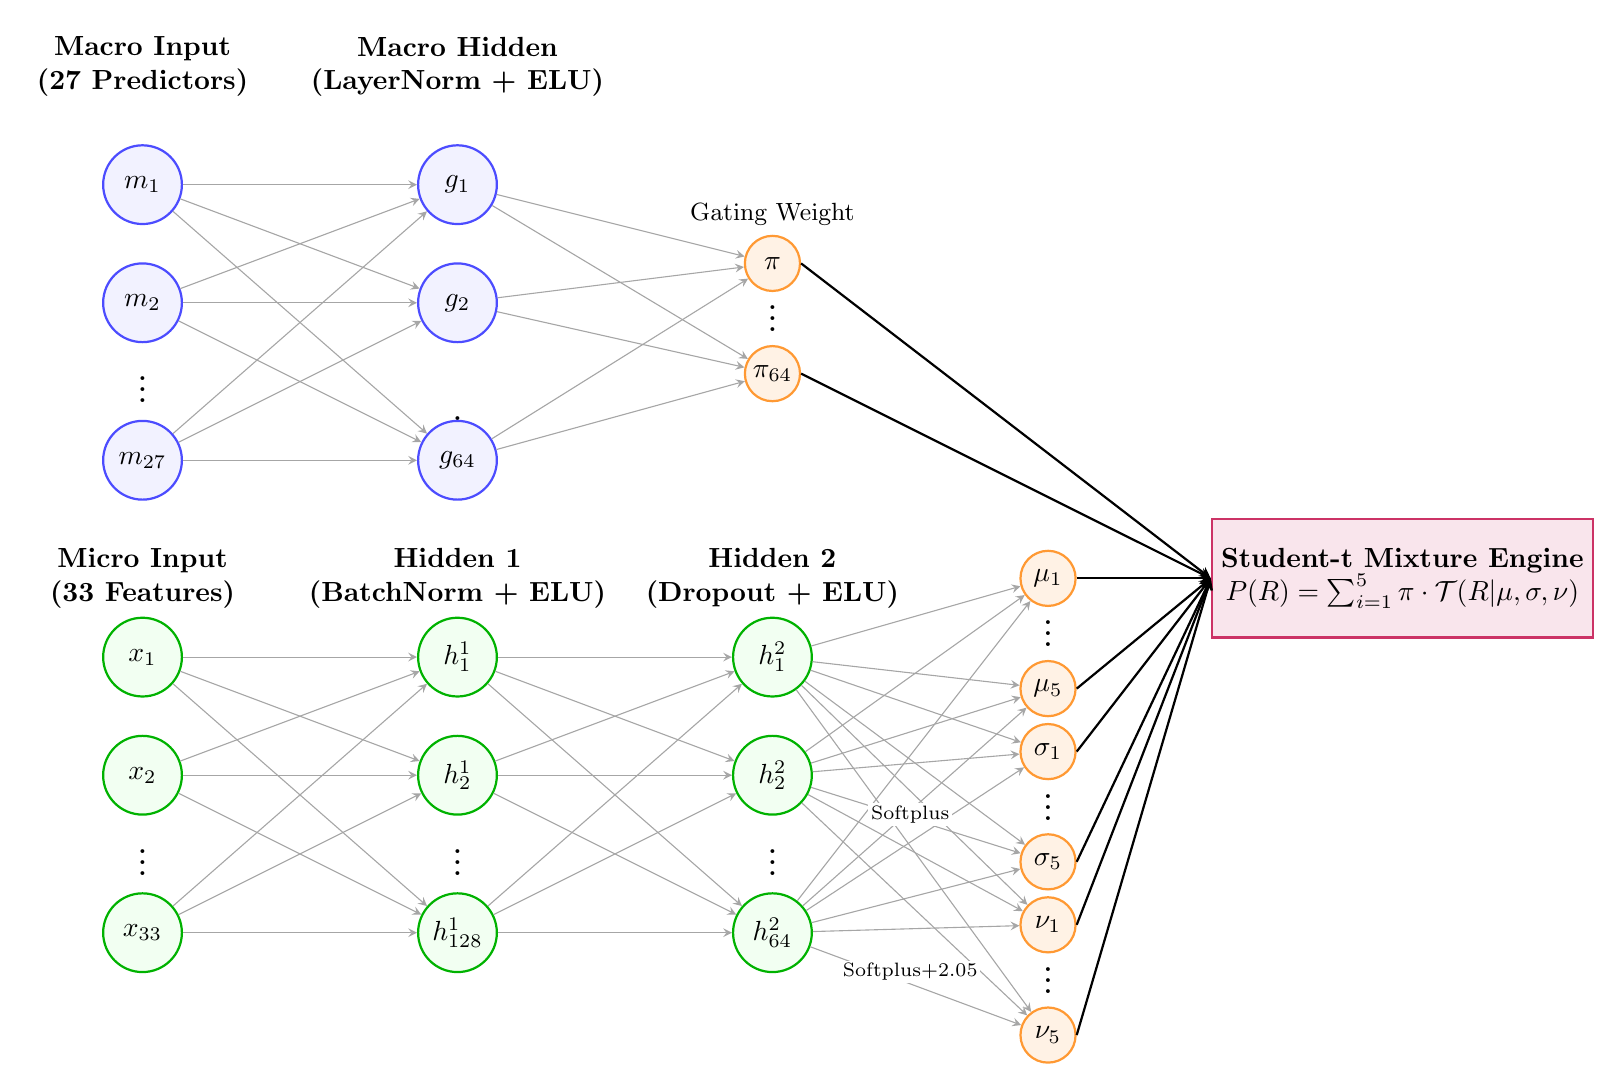
\begin{tikzpicture}[
        >=stealth, % 锐利的箭头
        macronode/.style={circle, draw=blue!70, fill=blue!5, thick, minimum size=10mm, inner sep=0pt},
        micronode/.style={circle, draw=green!70!black, fill=green!5, thick, minimum size=10mm, inner sep=0pt},
        paramnode/.style={circle, draw=orange!80, fill=orange!10, thick, minimum size=7mm, inner sep=0pt},
        engine/.style={rectangle, draw=purple!80, fill=purple!10, thick, minimum width=4cm, minimum height=1.5cm, align=center},
        output/.style={rectangle, draw=red!80, fill=red!10, thick, dashed, minimum width=4cm, minimum height=1.5cm, align=center},
        connect/.style={draw, ->, gray!70, thin}
    ]

    % ==========================================
    % 1. Macro Tower (Top Half)
    % ==========================================
    % 宏观输入层 (x=0)
    \node[macronode] (m1) at (0, 13) {$m_1$};
    \node[macronode] (m2) at (0, 11.5) {$m_2$};
    \node at (0, 10.5) {\Large $\vdots$};
    \node[macronode] (m27) at (0, 9.5) {$m_{27}$};
    \node[align=center, font=\bfseries] at (0, 14.5) {Macro Input\\(27 Predictors)};

    % 宏观隐藏层 (x=4)
    \node[macronode] (g1) at (4, 13) {$g_1$};
    \node[macronode] (g2) at (4, 11.5) {$g_2$};
    \node at (4, 10) {\Large $\vdots$};
    \node[macronode] (g64) at (4, 9.5) {$g_{64}$};
    \node[align=center, font=\bfseries] at (4, 14.5) {Macro Hidden\\(LayerNorm + ELU)};

    % 门控权重 (x=8)
    \node[paramnode] (pi1) at (8, 12) {$\pi$};
    \node at (8, 11.4) {\Large $\vdots$};
    \node[paramnode] (pi5) at (8, 10.6) {$\pi_{64}$};
    \node[above, font=\small] at (pi1.north) {Gating Weight};
    
    % 宏观直线连线 (绝对笔直)
    \foreach \i in {m1, m2, m27} {
        \foreach \j in {g1, g2, g64} {
            \path[connect] (\i) -- (\j);
        }
    }
    \path[connect] (g1) -- (pi1);
    \path[connect] (g2) -- (pi1);
    \path[connect] (g64) -- (pi1);
    \path[connect] (g1) -- (pi5);
    \path[connect] (g2) -- (pi5);
    \path[connect] (g64) -- (pi5);

    % ==========================================
    % 2. Micro Tower (Bottom Half)
    % ==========================================
    % 微观输入层 (x=0)
    \node[micronode] (x1) at (0, 7) {$x_1$};
    \node[micronode] (x2) at (0, 5.5) {$x_2$};
    \node at (0, 4.5) {\Large $\vdots$};
    \node[micronode] (x33) at (0, 3.5) {$x_{33}$};
    \node[align=center, font=\bfseries] at (0, 8) {Micro Input\\(33 Features)};

    % 隐藏层 1 (x=4)
    \node[micronode] (h1_1) at (4, 7) {$h^1_1$};
    \node[micronode] (h1_2) at (4, 5.5) {$h^1_2$};
    \node at (4, 4.5) {\Large $\vdots$};
    \node[micronode] (h1_128) at (4, 3.5) {$h^1_{128}$};
    \node[align=center, font=\bfseries] at (4, 8) {Hidden 1\\(BatchNorm + ELU)};

    % 隐藏层 2 (x=8)
    \node[micronode] (h2_1) at (8, 7) {$h^2_1$};
    \node[micronode] (h2_2) at (8, 5.5) {$h^2_2$};
    \node at (8, 4.5) {\Large $\vdots$};
    \node[micronode] (h2_64) at (8, 3.5) {$h^2_{64}$};
    \node[align=center, font=\bfseries] at (8, 8) {Hidden 2\\(Dropout + ELU)};

    % 分布参数 (x=11.5)
    \node[paramnode] (mu1) at (11.5, 8) {$\mu_1$};
    \node at (11.5, 7.4) {\Large $\vdots$};
    \node[paramnode] (mu5) at (11.5, 6.6) {$\mu_5$};
    \node[paramnode] (sigma1) at (11.5, 5.8) {$\sigma_1$};
    \node at (11.5, 5.2) {\Large $\vdots$};
    \node[paramnode] (sigma5) at (11.5, 4.4) {$\sigma_5$};
    \node[paramnode] (nu1) at (11.5, 3.6) {$\nu_1$};
    \node at (11.5, 3) {\Large $\vdots$};
    \node[paramnode] (nu5) at (11.5, 2.2) {$\nu_5$};

    % 微观直线连线 (绝对笔直)
    \foreach \i in {x1, x2, x33} {
        \foreach \j in {h1_1, h1_2, h1_128} {
            \path[connect] (\i) -- (\j);
        }
    }
    \foreach \i in {h1_1, h1_2, h1_128} {
        \foreach \j in {h2_1, h2_2, h2_64} {
            \path[connect] (\i) -- (\j);
        }
    }
    \foreach \i in {h2_1, h2_2, h2_64} {
        \path[connect] (\i) -- (mu1);
        \path[connect] (\i) -- (mu5);
        \path[connect] (\i) -- (sigma1);
        \path[connect] (\i) -- (sigma5);
        \path[connect] (\i) -- (nu1);
        \path[connect] (\i) -- (nu5);
    }
    
    % 在线上加上激活函数标注
    \node[fill=white, inner sep=1pt, font=\scriptsize] at (9.75, 5) {Softplus};
    \node[fill=white, inner sep=1pt, font=\scriptsize] at (9.75, 3) {Softplus+2.05};

    % ==========================================
    % 3. Mixture Engine & Output (Far Right)
    % ==========================================
    \node[engine] (mix) at (16, 8) {\textbf{Student-t Mixture Engine} \\ $P(R) = \sum_{i=1}^5 \pi \cdot \mathcal{T}(R | \mu, \sigma, \nu)$};
    % \node[output] (es) at (21.5, 6) {\textbf{5\% Expected Shortfall} \\ (ES)};

    % 连接到引擎 (虚线)
    \path[draw, ->, black, thick] (pi1.east) -- (mix.west);
    \path[draw, ->, black, thick] (pi5.east) -- (mix.west);
    \path[draw, ->, black, thick] (mu1.east) -- (mix.west);
    \path[draw, ->, black, thick] (mu5.east) -- (mix.west);
    \path[draw, ->, black, thick] (sigma1.east) -- (mix.west);
    \path[draw, ->, black, thick] (sigma5.east) -- (mix.west);
    \path[draw, ->, black, thick] (nu1.east) -- (mix.west);
    \path[draw, ->, black, thick] (nu5.east) -- (mix.west);
    
    % 引擎输出到 ES (加粗实线)
    % \path[draw, ->, black, very thick] (mix) -- (es);

    \end{tikzpicture}
    }
    \caption{Architecture of the Structured Mixture Density Network}
    \label{fig:fig_MDN_t}
\end{figure}

\textbf{1. The Macro Gating Network (Regime Channel):} 
The gating network takes the vector of macroeconomic predictors, $X_{t}^{macro}$, as input. It consists of a multi-layer perceptron (MLP) with Layer Normalization and Dropout to prevent overfitting to specific macro regimes. The output is a set of mixture weights, $\pi_{i,t,k}$, which represent the probability of the market being in a specific economic state or "regime" $k$ at time $t$:
\begin{equation}
    \pi_{i,t} = \text{Softmax}\Big( \text{MLP}_{macro}(X_{t}^{macro}) \Big)
\end{equation}
By relying exclusively on macroeconomic variables, the mixture weights $\pi$ are shared across all firms in a given cross-section, seamlessly capturing systemic regime shifts (e.g., transition from a bull market to a panic-driven crash).

\textbf{2. The Micro Expert Network (Firm-Specific Channel):}
The expert network processes the high-dimensional firm characteristics, $X_{i,t}^{micro}$. It utilizes Batch Normalization to accelerate cross-sectional convergence. For each firm $i$ and each regime $k$, the expert network outputs the location ($\mu$), scale ($\sigma$), and shape ($\nu$) parameters of the predictive distribution:
\begin{align}
    h_{i,t} &= \text{MLP}_{micro}(X_{i,t}^{micro}) \\
    \mu_{i,t,k} &= W_{\mu, k}^\top h_{i,t} + b_{\mu, k} \\
    \sigma_{i,t,k} &= \text{Softplus}\Big( W_{\sigma, k}^\top h_{i,t} + b_{\sigma, k} \Big) + \epsilon \\
    \nu_{i,t,k} &= \text{Softplus}\Big( W_{\nu, k}^\top h_{i,t} + b_{\nu, k} \Big) + 2.05 
\end{align}
To ensure numerical stability and economic validity, the scale parameter $\sigma$ is constrained to be strictly positive via a Softplus activation. Crucially, the degrees of freedom parameter $\nu$ is bounded below by $2.05$. In statistical theory, the variance of a Student-t distribution, $\frac{\nu}{\nu - 2}\sigma^2$, approaches infinity as $\nu \to 2$. Our imposed lower bound acts as an absolute physical firewall, ensuring that the conditional variance remains finite and preventing gradient explosions during optimization.

\subsection{The Student-t Mixture Engine}
\label{subsec:student_t}

A critical departure of our framework from standard MDNs is the choice of the base distribution. Financial returns are notoriously non-Gaussian, exhibiting excess kurtosis and extreme fat tails. A Gaussian Mixture Model (GMM) often requires an excessive number of components to approximate these tails, leading to severe overfitting in noisy financial datasets. 

Instead, we employ a Mixture of Student-t distributions. The conditional probability density of the one-month-ahead return, $R_{i,t+1}$, is modeled as:
\begin{equation}
    P(R_{i,t+1} | X_{t}^{macro}, X_{i,t}^{micro}) = \sum_{k=1}^{K} \pi_{t,k} \cdot \mathcal{T} \Big( R_{i,t+1} \Big| \mu_{i,t,k}, \sigma_{i,t,k}, \nu_{i,t,k} \Big)
\end{equation}
where $\mathcal{T}(\cdot)$ denotes the probability density function of the Student-t distribution. By endogenously learning the degrees of freedom $\nu_{i,t,k}$ from firm characteristics, our model can explicitly quantify whether a specific firm is prone to extreme tail realizations (low $\nu$) or exhibits stable, normal-like behaviors (high $\nu$).

\subsection{Objective Function and Time-Decay Weighting}
\label{subsec:objective}

The model is optimized by minimizing the Negative Log-Likelihood (NLL) of the realized returns. Furthermore, recognizing that financial markets are non-stationary and that recent observations carry more relevant information about the current economic state than distant ones, we introduce an exponential time-decay weighting scheme. 

The loss function for a given training window is defined as:
\begin{equation}
    \mathcal{L} = - \frac{1}{N \times T} \sum_{t=1}^{T} \sum_{i=1}^{N} w_{t} \log \left( \sum_{k=1}^{K} \pi_{t,k} \cdot \mathcal{T}(R_{i,t+1} | \mu_{i,t,k}, \sigma_{i,t,k}, \nu_{i,t,k}) \right)
\end{equation}
where $w_{t}$ is the time-decay weight, calculated as $w_{t} \propto 0.5^{\frac{\Delta m}{H}}$, with $\Delta m$ being the number of months between time $t$ and the end of the current training window, and $H$ being the half-life parameter (e.g., 36 months). The weights are normalized such that their mean equals 1, ensuring a consistent gradient magnitude.

\subsection{Expanding Window and Warm-Start Optimization}
\label{subsec:optimization}

To strictly avoid look-ahead bias and simulate real-world trading constraints, we train the Structured MDN using an expanding window walk-forward approach. The initial model is trained on the first 15 years of data. Subsequently, the window rolls forward by one year at a time.

A key methodological innovation in our pipeline is the use of \textbf{Warm-Start Fine-Tuning}. Instead of re-initializing the neural network weights randomly for each new window, the model inherits the converged weights from the previous window. This mechanism serves two critical purposes:
\begin{enumerate}
    \item \textbf{Economic Consistency:} It endogenously replicates the classical asset pricing assumption that the underlying mapping functions of Alphas and conditional Betas evolve slowly over time, effectively acting as an implicit time-domain smoothing filter.
    \item \textbf{Preventing Catastrophic Forgetting:} During the fine-tuning phase of each new window, we combine the newly available data with the historical training set to update the gradients. This prevents the deep neural network from "catastrophically forgetting" the long-term structural relationships (e.g., past financial crises) when exposed to a new, short-term localized regime.
\end{enumerate}
Through this robust optimization protocol, the model continuously adapts to the freshest macroeconomic states while maintaining a deep memory of historical crash dynamics.


\section{Density Forecast Evaluation}
\label{sec:evaluation}

Evaluating a density forecast is inherently more complex than assessing point forecasts, as the "true" probability distribution is never directly observable. To rigorously validate the predictive performance of our Structured MDN, we employ two complementary frameworks: global calibration checks via the Probability Integral Transform (PIT) and accuracy scoring via the Continuous Ranked Probability Score (CRPS).

\subsection{Calibration and Probability Integral Transform (PIT)}
\label{subsec:pit}

A predictive density is said to be "well-calibrated" if the realized observations are statistically consistent with the forecasted distribution. We assess this using the Probability Integral Transform (PIT), defined as the cumulative distribution function (CDF) of the forecast evaluated at the realized return $R_{i,t+1}$:
\begin{equation}
    Z_{i,t+1} = \int_{-\infty}^{R_{i,t+1}} \hat{p}(x | X_{t}^{macro}, X_{i,t}^{micro}) \, dx = \hat{F}(R_{i,t+1} | \mathcal{F}_t)
\end{equation}
Under the null hypothesis that the model is correctly specified, the PIT values should be independent and identically distributed as $U(0, 1)$ . 

\begin{figure}[htbp]
    \caption{PIT and QQ-plot}
    \label{fig:fig_pit_qqplot}
    \centering

	\subfloat[PIT]{
	    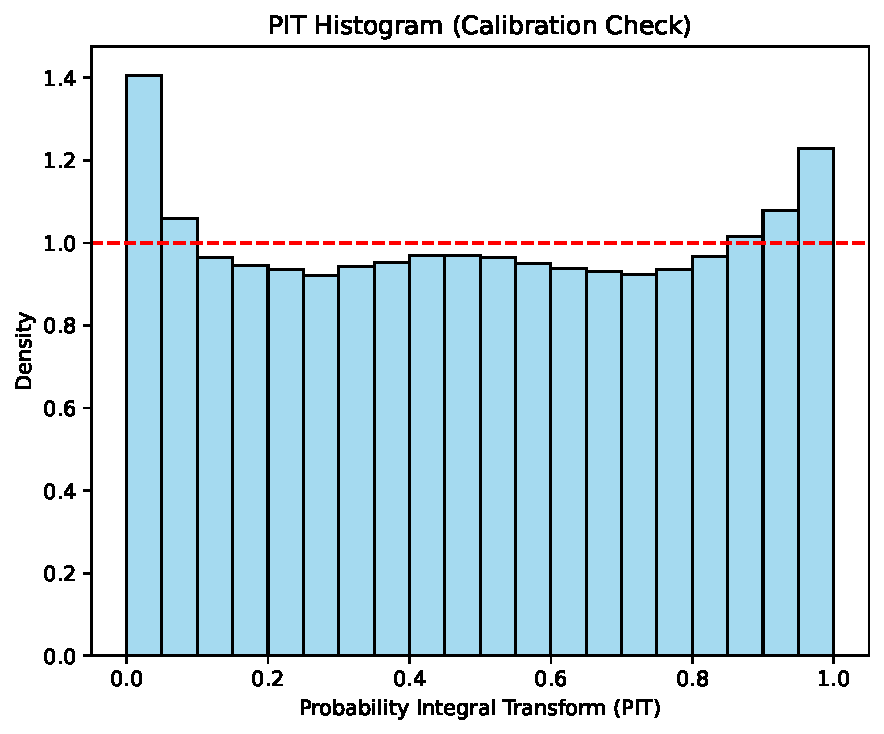
\includegraphics[width=0.48\textwidth]{fig/pit_histogram.pdf}
	 }
	\subfloat[QQ-plot]{
	    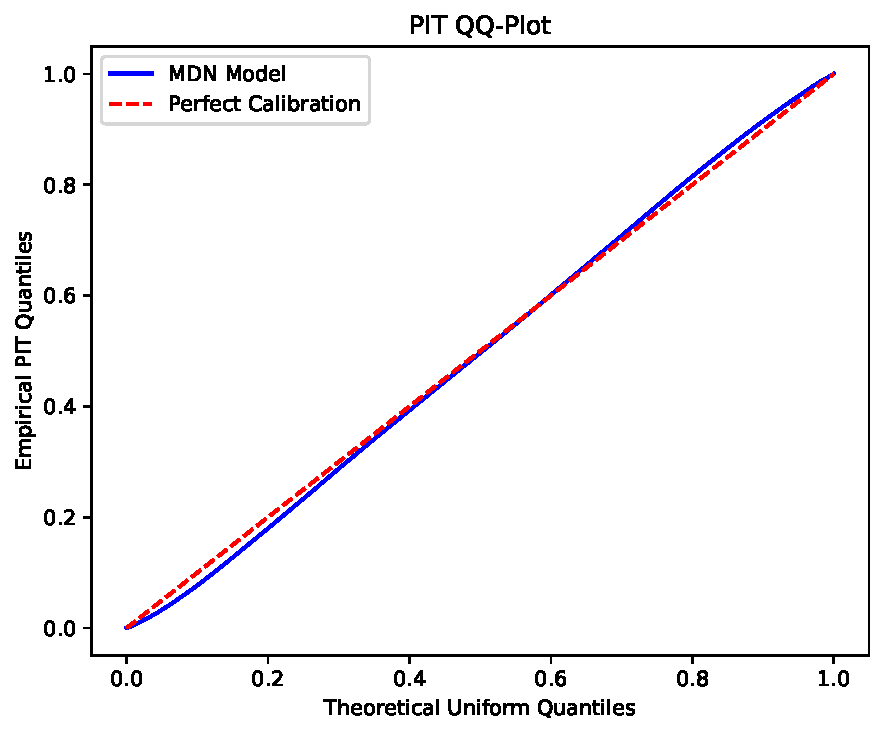
\includegraphics[width=0.48\textwidth]{fig/pit_qq_plot.pdf}
	 }
    % \vspace{0.2cm}
 %    \begin{minipage}{0.95\textwidth} 
	% {\footnotesize Now see how we can have two panels! \ldots
	% \par
	% }
	% \end{minipage}
\end{figure}




% \begin{figure}[htbp]
%     \centering
    
%     % 左图
%     \begin{minipage}[b]{0.48\textwidth}
%         \centering
%         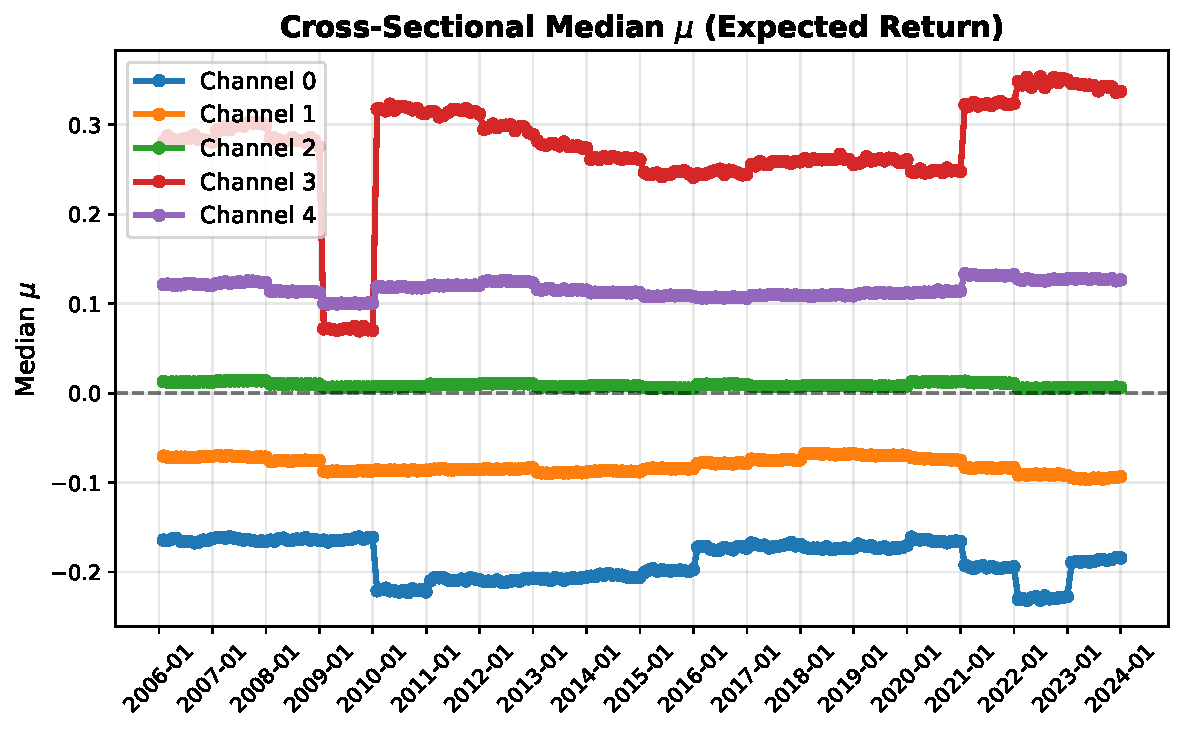
\includegraphics[width=\textwidth]{fig/regime_mu_all.pdf}
%         \vspace{0.1cm}
%         \centerline{(a) Title of Left Figure}
%     \end{minipage}
%     \hfill
%     % 右图
%     \begin{minipage}[b]{0.48\textwidth}
%         \centering
%         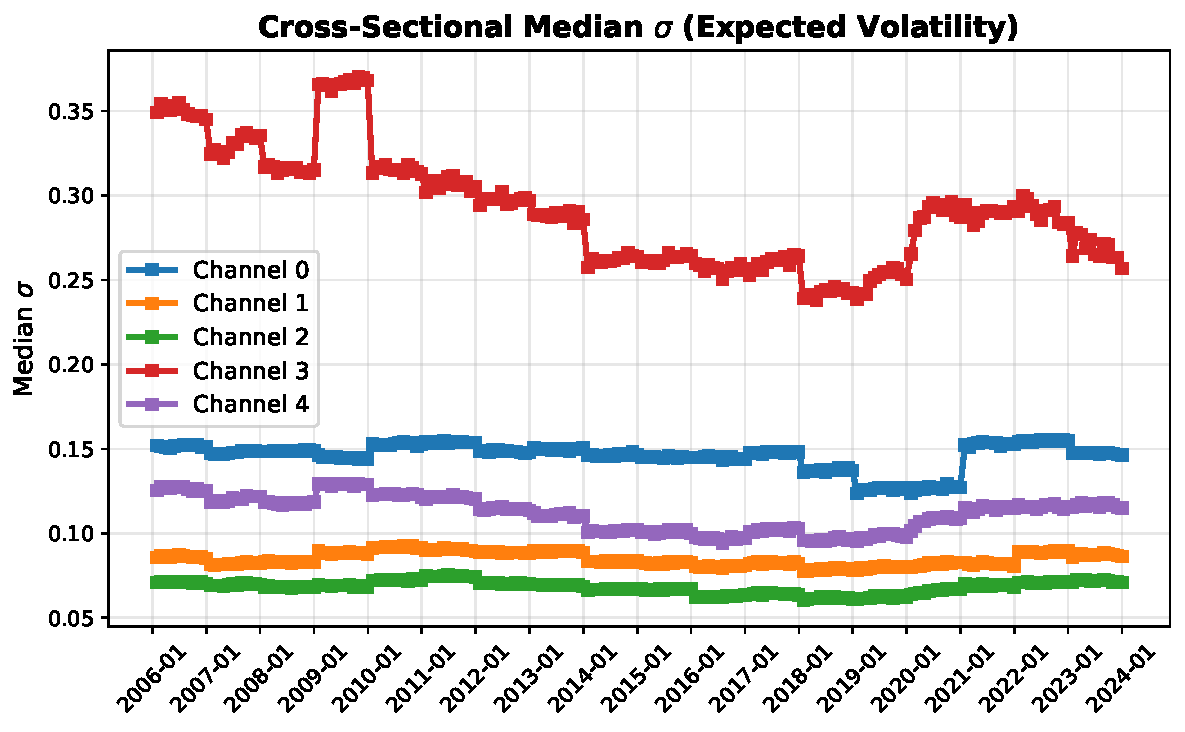
\includegraphics[width=\textwidth]{fig/regime_sigma_all.pdf}
%         \vspace{0.1cm}
%         \centerline{(b) Title of Right Figure}
%     \end{minipage}
    
%     \caption{This is the main caption for both figures.}
%     \label{fig:fig_pit_qqplot}
% \end{figure}

Figure \ref{fig:fig_pit_qqplot} presents the PIT histogram and QQ-plot for our Sample-Out-of-Sample (OOS) period. The QQ-plot exhibits a blue line that closely tracks the 45-degree diagonal, indicating that the MDN provides a globally unbiased estimation of the conditional return density. The PIT histogram shows a nearly uniform distribution with a slight, symmetrical "U-shape" at the extreme tails. This minor "smile" pattern suggests a slight under-dispersion, likely driven by unforecastable idiosyncratic shocks or extreme black-swan events that exceed even the heavy-tailed Student-t specification. However, compared to standard Gaussian benchmarks, the MDN demonstrates superior tail-capture capabilities.

\subsection{Predictive Accuracy and Scoring Rules}
\label{subsec:crps}

While PIT measures the "reliability" of the distribution, it does not measure its "sharpness" (precision). To evaluate the overall quality of the density forecast, we use the \textbf{Continuous Ranked Probability Score (CRPS)}, which is a proper scoring rule that penalizes both lack of calibration and excessive variance. The CRPS is defined as:
\begin{equation}
    \text{CRPS}(F, y) = \int_{-\infty}^{\infty} [F(x) - \mathbb{I}(x \geq y)]^2 \, dx
\end{equation}
where $F$ is the predicted CDF and $\mathbb{I}(\cdot)$ is the indicator function. Unlike the Negative Log-Likelihood (NLL), which can be overly sensitive to extreme outliers, CRPS is robust and has the same unit as the realized return, making it economically interpretable.

We calculate the CRPS for our Student-t mixture using the analytical solution derived by . To demonstrate the incremental value of our deep learning approach, we compare the MDN's performance against two benchmarks:
\begin{enumerate}
    \item \textbf{Historical Normal (Benchmark):} A rolling 12-month historical mean and volatility model.
    \item \textbf{Linear Quantile Regression (LQR):} A semi-parametric baseline that estimates 99 discrete quantiles using the same feature set.
\end{enumerate}

\begin{figure}[htbp]
    \begin{center}
    \caption{crps comparison}
    \label{fig:fig_crps_comparison}
    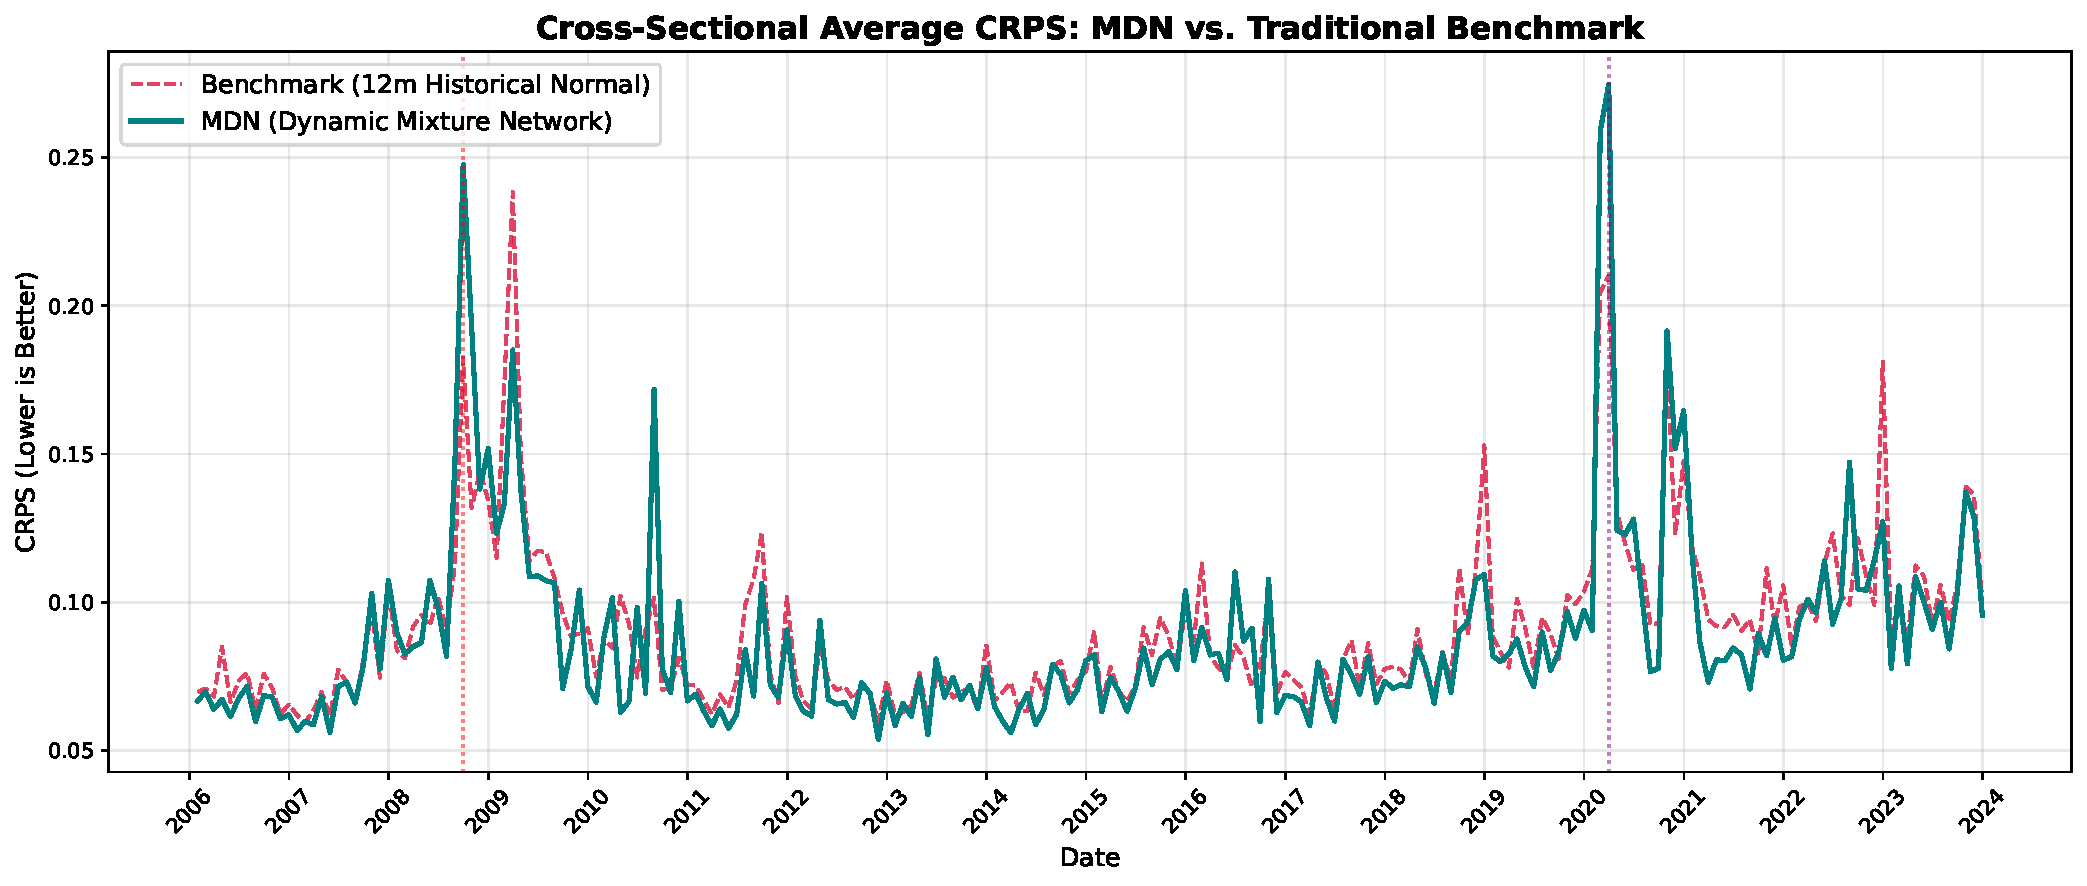
\includegraphics[width=1\textwidth]{fig/crps_comparison.pdf}
    \end{center}
    % \vspace{0.2cm}
 %    \begin{minipage}{0.95\textwidth} 
	% {\footnotesize This figure plots \ldots
	% \par
	% }
	% \end{minipage}
\end{figure}


To quantify the improvement, we define the \textbf{MDN Skill Score} as the percentage reduction in CRPS relative to the traditional benchmark:
\begin{equation}
    \text{Skill Score} = \left( 1 - \frac{\text{CRPS}_{\text{MDN}}}{\text{CRPS}_{\text{Bench}}} \right) \times 100\%
\end{equation}
Our empirical results show that the Structured MDN consistently achieves a positive Skill Score, particularly during high-volatility regimes such as the 2008 Financial Crisis and the 2020 COVID-19 crash. This superiority stems from the model's ability to utilize macroeconomic state variables to dynamically adjust mixture weights, thereby capturing non-linear regime shifts that are invisible to rolling historical windows or linear quantile models.

\subsection{Evolution of Regime Dynamics}



\begin{figure}[htbp]
    \centering
    % 左图：Mu 的演化
    \begin{minipage}[b]{0.48\textwidth}
        \centering
        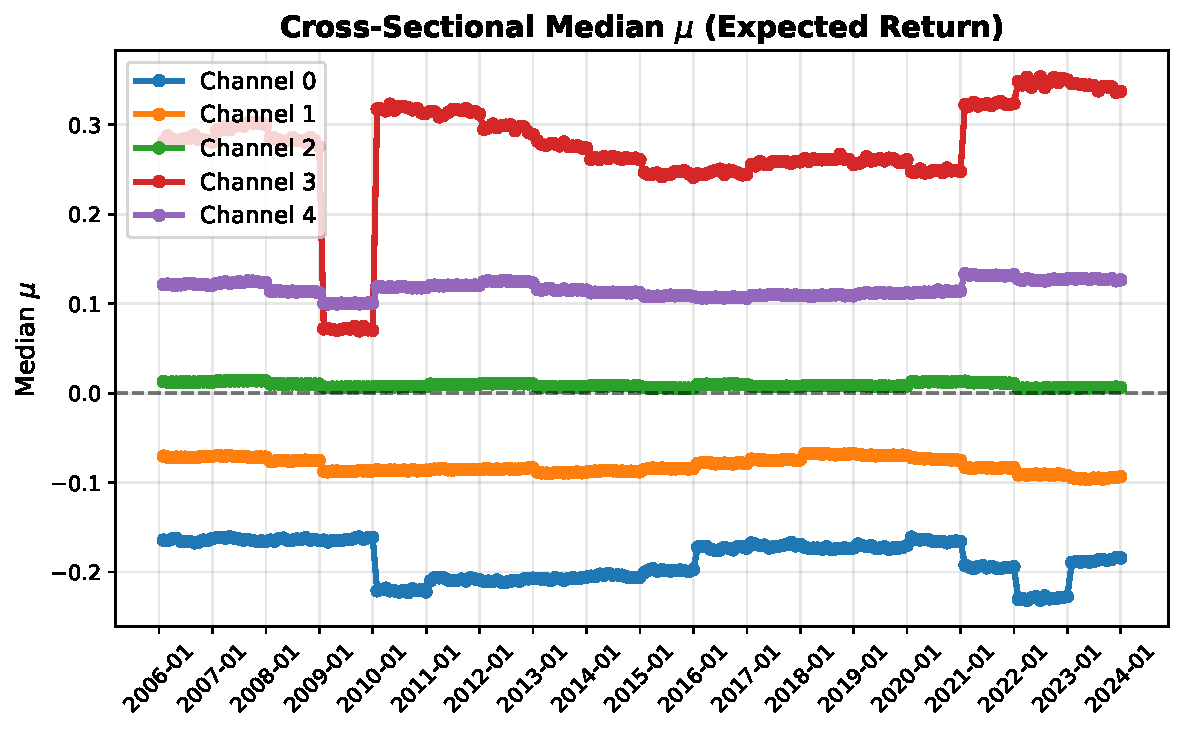
\includegraphics[width=\textwidth]{fig/regime_mu_all.pdf}
        % \caption{Dynamics of Conditional Mean ($\mu$)}
        % \label{fig:regime_mu}
    \end{minipage}
    \hfill
    % 右图：Sigma 的演化
    \begin{minipage}[b]{0.48\textwidth}
        \centering
        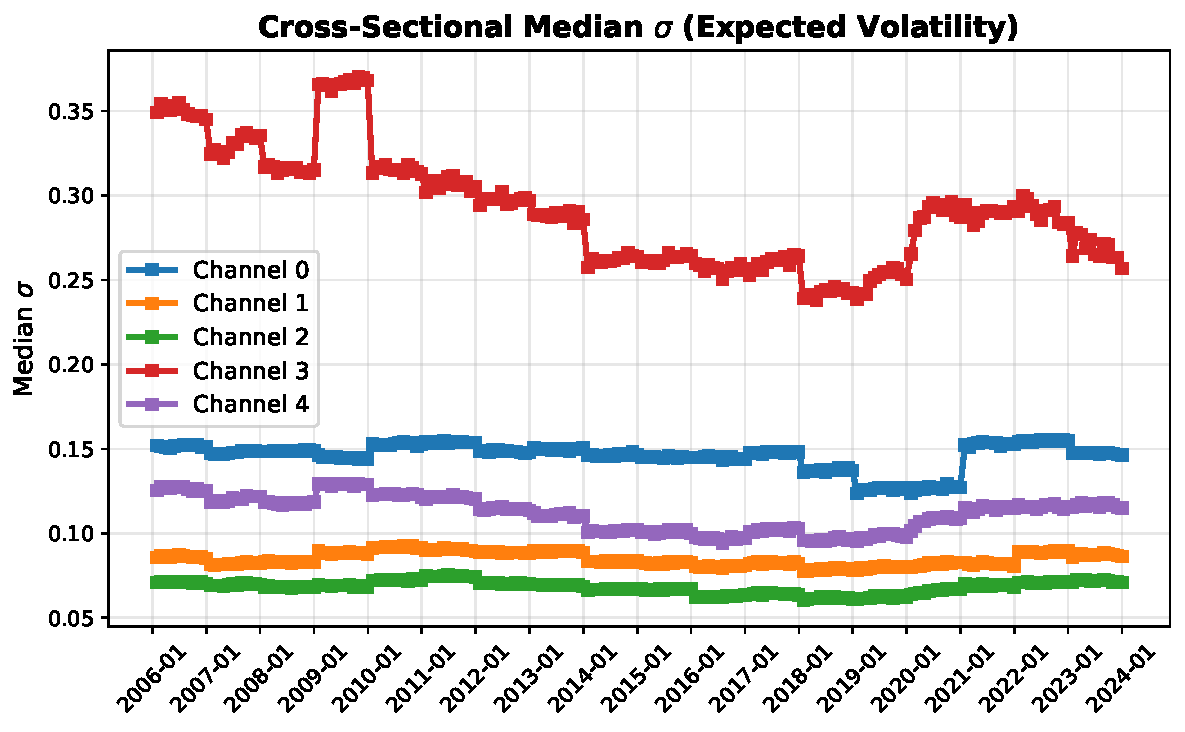
\includegraphics[width=\textwidth]{fig/regime_sigma_all.pdf}
        % \caption{Dynamics of Conditional Volatility ($\sigma$)}
        % \label{fig:regime_sigma}
    \end{minipage}
    
    \caption{Evolution of Regime Dynamics. This figure plots the cross-sectional medians of the component-specific expected returns (Panel a) and expected volatilities (Panel b) extracted from the micro expert network. Each line represents a distinct underlying market regime dynamically tracked by the model over time.}
    \label{fig:fig_regime_mu_sigma}
\end{figure}

\section{Asset Pricing Tests}
\label{sec:asset_pricing_tests}

In this section, we formally evaluate the cross-sectional pricing power of the conditional tail risk—specifically, the 5\% Expected Shortfall ($ES_{i,t}$) predicted by our Structured Mixture Density Network (MDN). Consistent with the theoretical framework established in Section X, which suggests that investors demand a premium for bearing extreme downside risk, we test whether stocks with higher MDN-implied $ES_{i,t}$ earn higher subsequent expected returns. We employ three standard empirical asset pricing methodologies: univariate decile portfolio sorts, Fama-MacBeth cross-sectional regressions, and time-series factor spanning tests.

\subsection{Univariate Decile Portfolio Sorts}
\label{subsec:decile_sorts}

We begin by examining the unadjusted relationship between the predicted tail risk and future stock returns through non-parametric portfolio sorts. At the end of each month $t$, we sort all eligible stocks into ten decile portfolios based on their out-of-sample MDN-predicted $ES_{i,t}$. Decile 1 (Low ES) contains stocks with the lowest predicted tail risk, while Decile 10 (High ES) contains stocks with the highest predicted tail risk. 

We compute the value-weighted (and equal-weighted, for robustness) returns for each decile portfolio over the subsequent holding period, month $t+1$. To capture the tail risk premium, we construct a zero-investment long-short portfolio (High-minus-Low) that goes long the stocks in Decile 10 and short the stocks in Decile 1. 

If the MDN accurately isolates priced tail risk, we hypothesize a monotonically increasing pattern in the post-formation realized returns from Decile 1 to Decile 10, culminating in a statistically significant and economically meaningful positive spread for the High-minus-Low portfolio.

\subsection{Fama-MacBeth Cross-Sectional Regressions}
\label{subsec:fama_macbeth}

While portfolio sorts provide intuitive evidence of a risk premium, they cannot simultaneously control for a multitude of firm characteristics that are known to predict the cross-section of returns. To rigorously isolate the marginal pricing information embedded in our MDN-predicted $ES_{i,t}$, we employ the cross-sectional regression methodology of Fama and MacBeth (1973). 

For each month $t$, we estimate the following cross-sectional ordinary least squares (OLS) regression:
\begin{equation}
    R_{i,t+1} = \gamma_{0,t} + \gamma_{1,t} ES_{i,t} + \boldsymbol{\Gamma}_t^{\top} \mathbf{X}_{i,t} + \epsilon_{i,t+1}
\end{equation}
where $R_{i,t+1}$ is the realized excess return of stock $i$ in month $t+1$. The key independent variable is our machine-learning-derived $ES_{i,t}$. The vector $\mathbf{X}_{i,t}$ incorporates a comprehensive set of standard firm-level control variables, including firm size (Log ME), book-to-market ratio (BM), short-term reversal ($Ret_{-1}$), momentum ($Ret_{-12,-2}$), and illiquidity (Amihud).

Following the standard procedure, we aggregate the time-series of the estimated monthly coefficients ($\hat{\gamma}_{1,t}$) to calculate their time-series averages. Statistical significance is assessed using Newey-West (1987) standard errors to account for potential autocorrelation and heteroskedasticity in the coefficient series. A significantly positive time-series average of $\hat{\gamma}_{1,t}$ would confirm that the tail risk premium remains robust after controlling for well-established market anomalies.

\subsection{Time-Series Factor Spanning Tests (Portfolio Alphas)}
\label{subsec:spanning_tests}

To further ensure that the excess returns generated by the $ES_{i,t}$-sorted portfolios are not merely compensations for exposures to existing systematic risk factors, we perform time-series factor spanning tests. We regress the time-series of the High-minus-Low zero-investment portfolio returns on standard asset pricing factor models.

Specifically, we utilize the Fama-French five-factor model (Fama and French, 2015) augmented with the momentum factor (Carhart, 1997):
\begin{equation}
\begin{aligned}
    R_{High,t} - R_{Low,t} &= \alpha + \beta_{MKT} MKT_t + \beta_{SMB} SMB_t + \beta_{HML} HML_t \\
    &\quad + \beta_{RMW} RMW_t + \beta_{CMA} CMA_t + \beta_{UMD} UMD_t + \varepsilon_t
\end{aligned}
\end{equation}
The intercept of this regression, $\alpha$, represents the risk-adjusted abnormal return. A statistically significant and positive $\alpha$ indicates that the MDN-implied tail risk premium is orthogonal to the traditional factor space. In other words, the deep learning model successfully extracts a novel dimension of risk that traditional linear factor models fail to span.

\section{Additional Robustness \& Extensions}

\section{Conclusion}


\section{Results \label{sec:results}}




% \input{tab_tex/summary_stats.tex}


% Table \ref{tab:summary_stats} 

% \input{fig_tex/fig_mainsummary.tex}

% Figure \ref{fig:fig_mainsummary} .

% \input{tab_tex/regressions.tex}

% The top panel of Table \ref{tab:regressions} 

\section{Conclusion \label{sec:conclusion}}






%%%%%%%%%%%%%%%%%%%%%%%%%%%%%%%%%%%%%%%%%%%%%%%%%
\clearpage
\begin{singlespace}
%\bibliographystyle{plainnat}
%\bibliographystyle{chicago}
\bibliographystyle{aer}
\bibliography{our-cites.bib}
\end{singlespace}
%%%%%%%%%%%%%%%%%%%%%%%%%%%%%%%%%%%%%%%%%%%%%%%%%


%%%%%%%%%%%%%%%%%%%%%%%%%%%%%%%%%%%%%%%%%%%%%%%%%
%%%%% These commands start the appendix and change the Table & Figure numbering
\newpage
\appendix
\setcounter{table}{0}
\renewcommand{\tablename}{Appendix Table}
\renewcommand{\figurename}{Appendix Figure}
\renewcommand{\thetable}{A\arabic{table}}
\setcounter{figure}{0}
\renewcommand{\thefigure}{A\arabic{figure}}
%%%%%%%%%%%%%%%%%%%%%%%%%%%%%%%%%%%%%%%%%%%%%%%%%

\section{Appendix Tables and Figures}
% \input{tab_tex/other-regressions.tex}

\newpage 
\section{Appendix One \label{sec:appendix:first}}
\renewcommand{\thetable}{B\arabic{table}}
\setcounter{table}{0}
\renewcommand{\thefigure}{B\arabic{figure}}
\setcounter{figure}{0}

A

\begin{figure}[htbp]
    \centering
    % 根据页面宽度自动缩放，保证不超页边距
    \resizebox{\textwidth}{!}{
    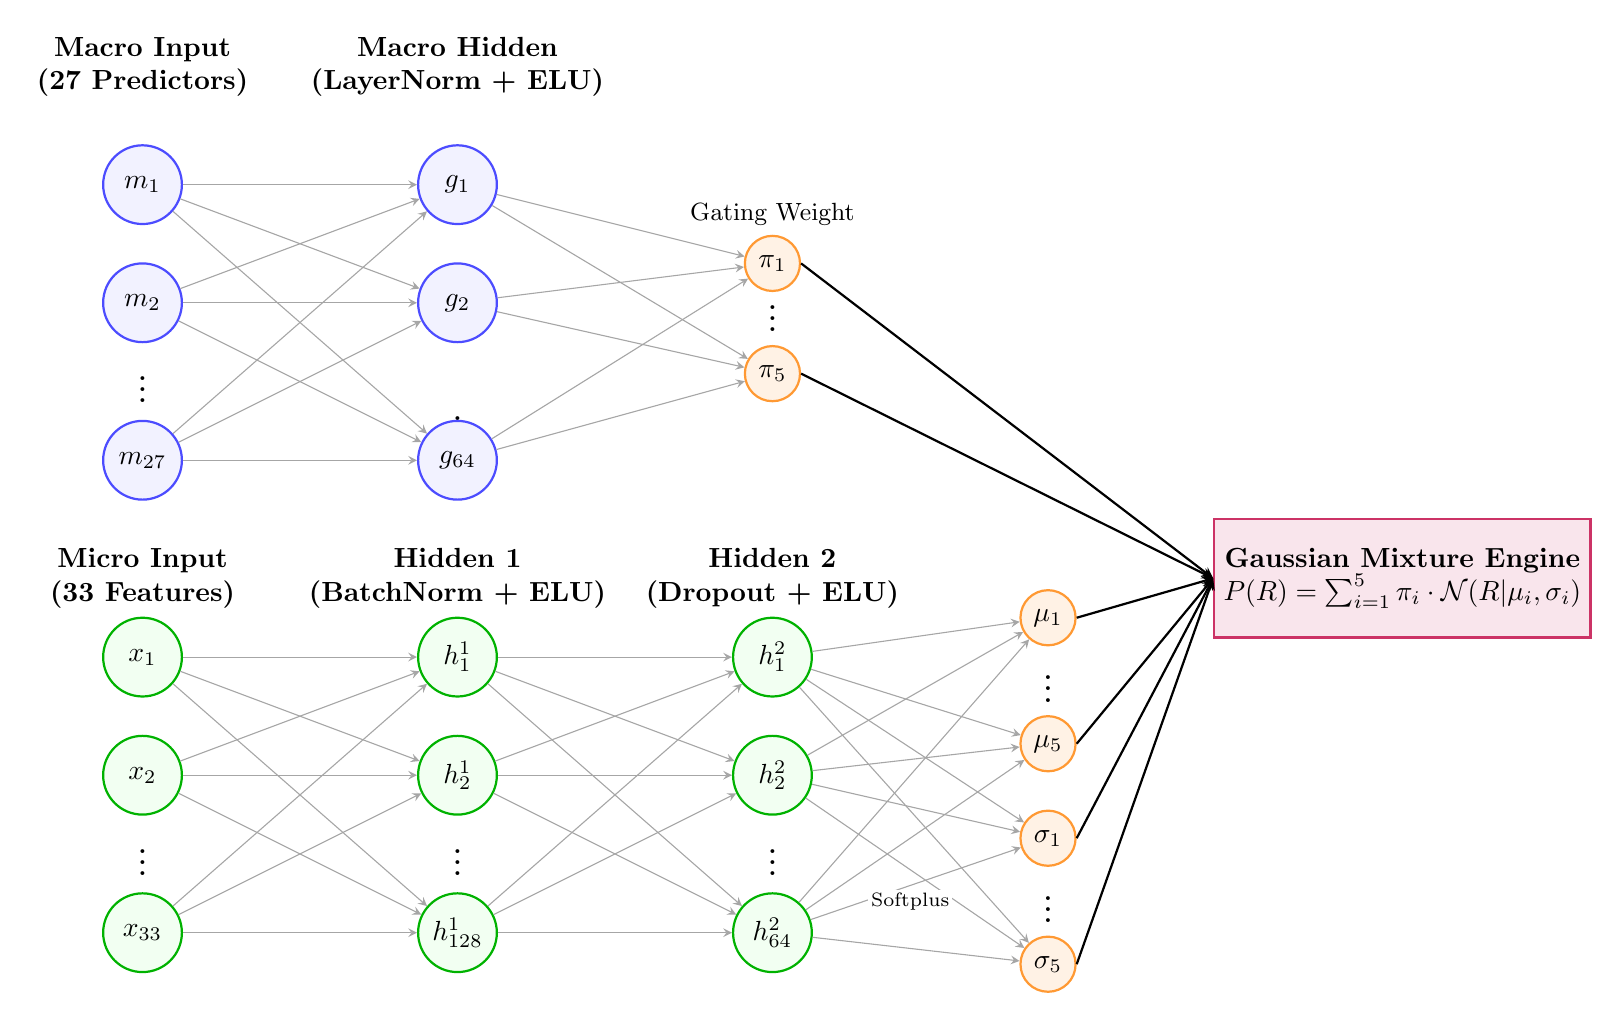
\begin{tikzpicture}[
        >=stealth, % 锐利的箭头
        macronode/.style={circle, draw=blue!70, fill=blue!5, thick, minimum size=10mm, inner sep=0pt},
        micronode/.style={circle, draw=green!70!black, fill=green!5, thick, minimum size=10mm, inner sep=0pt},
        paramnode/.style={circle, draw=orange!80, fill=orange!10, thick, minimum size=7mm, inner sep=0pt},
        engine/.style={rectangle, draw=purple!80, fill=purple!10, thick, minimum width=4cm, minimum height=1.5cm, align=center},
        output/.style={rectangle, draw=red!80, fill=red!10, thick, dashed, minimum width=4cm, minimum height=1.5cm, align=center},
        connect/.style={draw, ->, gray!70, thin}
    ]

    % ==========================================
    % 1. Macro Tower (Top Half)
    % ==========================================
    % 宏观输入层 (x=0)
    \node[macronode] (m1) at (0, 13) {$m_1$};
    \node[macronode] (m2) at (0, 11.5) {$m_2$};
    \node at (0, 10.5) {\Large $\vdots$};
    \node[macronode] (m27) at (0, 9.5) {$m_{27}$};
    \node[align=center, font=\bfseries] at (0, 14.5) {Macro Input\\(27 Predictors)};

    % 宏观隐藏层 (x=4)
    \node[macronode] (g1) at (4, 13) {$g_1$};
    \node[macronode] (g2) at (4, 11.5) {$g_2$};
    \node at (4, 10) {\Large $\vdots$};
    \node[macronode] (g64) at (4, 9.5) {$g_{64}$};
    \node[align=center, font=\bfseries] at (4, 14.5) {Macro Hidden\\(LayerNorm + ELU)};

    % 门控权重 (x=8)
    \node[paramnode] (pi1) at (8, 12) {$\pi_1$};
    \node at (8, 11.4) {\Large $\vdots$};
    \node[paramnode] (pi5) at (8, 10.6) {$\pi_5$};
    \node[above, font=\small] at (pi1.north) {Gating Weight};
    
    % 宏观直线连线 (绝对笔直)
    \foreach \i in {m1, m2, m27} {
        \foreach \j in {g1, g2, g64} {
            \path[connect] (\i) -- (\j);
        }
    }
    \path[connect] (g1) -- (pi1);
    \path[connect] (g2) -- (pi1);
    \path[connect] (g64) -- (pi1);
    \path[connect] (g1) -- (pi5);
    \path[connect] (g2) -- (pi5);
    \path[connect] (g64) -- (pi5);

    % ==========================================
    % 2. Micro Tower (Bottom Half)
    % ==========================================
    % 微观输入层 (x=0)
    \node[micronode] (x1) at (0, 7) {$x_1$};
    \node[micronode] (x2) at (0, 5.5) {$x_2$};
    \node at (0, 4.5) {\Large $\vdots$};
    \node[micronode] (x33) at (0, 3.5) {$x_{33}$};
    \node[align=center, font=\bfseries] at (0, 8) {Micro Input\\(33 Features)};

    % 隐藏层 1 (x=4)
    \node[micronode] (h1_1) at (4, 7) {$h^1_1$};
    \node[micronode] (h1_2) at (4, 5.5) {$h^1_2$};
    \node at (4, 4.5) {\Large $\vdots$};
    \node[micronode] (h1_128) at (4, 3.5) {$h^1_{128}$};
    \node[align=center, font=\bfseries] at (4, 8) {Hidden 1\\(BatchNorm + ELU)};

    % 隐藏层 2 (x=8)
    \node[micronode] (h2_1) at (8, 7) {$h^2_1$};
    \node[micronode] (h2_2) at (8, 5.5) {$h^2_2$};
    \node at (8, 4.5) {\Large $\vdots$};
    \node[micronode] (h2_64) at (8, 3.5) {$h^2_{64}$};
    \node[align=center, font=\bfseries] at (8, 8) {Hidden 2\\(Dropout + ELU)};

    % 分布参数 (x=11.5) - 重新调整了 Y 坐标以保持垂直居中
    \node[paramnode] (mu1) at (11.5, 7.5) {$\mu_1$};
    \node at (11.5, 6.7) {\Large $\vdots$};
    \node[paramnode] (mu5) at (11.5, 5.9) {$\mu_5$};
    \node[paramnode] (sigma1) at (11.5, 4.7) {$\sigma_1$};
    \node at (11.5, 3.9) {\Large $\vdots$};
    \node[paramnode] (sigma5) at (11.5, 3.1) {$\sigma_5$};

    % 微观直线连线 (绝对笔直)
    \foreach \i in {x1, x2, x33} {
        \foreach \j in {h1_1, h1_2, h1_128} {
            \path[connect] (\i) -- (\j);
        }
    }
    \foreach \i in {h1_1, h1_2, h1_128} {
        \foreach \j in {h2_1, h2_2, h2_64} {
            \path[connect] (\i) -- (\j);
        }
    }
    \foreach \i in {h2_1, h2_2, h2_64} {
        \path[connect] (\i) -- (mu1);
        \path[connect] (\i) -- (mu5);
        \path[connect] (\i) -- (sigma1);
        \path[connect] (\i) -- (sigma5);
    }
    
    % 在线上加上激活函数标注 (位置同步下移对齐 sigma)
    \node[fill=white, inner sep=1pt, font=\scriptsize] at (9.75, 3.9) {Softplus};

    % ==========================================
    % 3. Mixture Engine & Output (Far Right)
    % ==========================================
    \node[engine] (mix) at (16, 8) {\textbf{Gaussian Mixture Engine} \\ $P(R) = \sum_{i=1}^5 \pi_i \cdot \mathcal{N}(R | \mu_i, \sigma_i)$};

    % 连接到引擎 (实线加粗)
    \path[draw, ->, black, thick] (pi1.east) -- (mix.west);
    \path[draw, ->, black, thick] (pi5.east) -- (mix.west);
    \path[draw, ->, black, thick] (mu1.east) -- (mix.west);
    \path[draw, ->, black, thick] (mu5.east) -- (mix.west);
    \path[draw, ->, black, thick] (sigma1.east) -- (mix.west);
    \path[draw, ->, black, thick] (sigma5.east) -- (mix.west);
    
    \end{tikzpicture}
    }
    \caption{Architecture of the Structured Gaussian Mixture Density Network}
    \label{fig:fig_MDN_N}
\end{figure}
\ref{fig:fig_MDN_N}

\newpage
\section{Appendix Two \label{sec:appendix:two}}
\renewcommand{\thetable}{C\arabic{table}}
\setcounter{table}{0}
\renewcommand{\thefigure}{C\arabic{figure}}
\setcounter{figure}{0}

B



\end{document}
